%% Follow comments to support use.

%%%%%%%%%%%%%%%%%%%%%%%%%%%%%%%%%%%%%%%%%%%%%%%%%%%%%%%%%
%% STEP 1: Choose options for MSc / BSc / seminar layout and your bibliographic style
%%%%%%%%%%%%%%%%%%%%%%%%%%%%%%%%%%%%%%%%%%%%%%%%%%%%%%%%%

%%  Language: 
%%      finnish, swedish, or english
%%  Pagination (use twoside by default)  
%%      oneside or twoside,
%%  Study programme / kind of report
%%      csm  = Master's thesis in Computer Science Master's Programme;
%%      tkt = Bachelor's thesis in Computer Science Bachelor's Programme;
%%      seminar = seminar report
%%  For Master's thesis choose your line or track:
%%      (30 cr thesis, 2020 onwards, Master's Programme in Computer Science = csm)
%%      software-track-2020 = Software study track
%%      algorithms-track-2020 = Algorithms study track
%%      networking-track-2020 = Networking study track

\documentclass[finnish,oneside,censored,tkt,software-track-2020]{HYthesisML} 


% If wanted, open new chapters only at right page.
% By default, "openany".
%\PassOptionsToClass{openright,twoside,a4paper}{report}
\PassOptionsToClass{openany,oneside,a4paper}{report}

\usepackage{csquotes}
%%%%%%%%%%%%%%%%%%%%%%%%%%%%%%%%%%%%%%%%%%%%%%%%%%%%%%%%%
%% REFERENCES
%% Some notes on bibliography usage and options:
%% natbib -> you can use, e.g., \citep{} or \parencite{} for (Einstein, 1905); with APA \cite -> Einstein, 1905 without ()
%% maxcitenames=2 -> only 2 author names in text citations, if more -> et al. is used
%% maxbibnames=99 as no great need to suppress the biliography list in a thesis
%% for more information see biblatex package documentation, e.g., from https://ctan.org/pkg/biblatex 

%% Reference style: select one 
%% for APA = Harvard style = authoryear -> (Einstein, 1905) use:
%\usepackage[style=authoryear,bibstyle=authoryear,backend=biber,natbib=true,maxnames=99,maxcitenames=2,uniquelist=minyear,giveninits=true,uniquename=mininit]{biblatex}
%% for numeric = Vancouver style -> [1] use:
\usepackage[style=numeric,bibstyle=numeric,backend=biber,natbib=true,maxbibnames=99,giveninits=true,uniquename=init]{biblatex}
%% for alpahbetic -> [Ein05] use:
%\usepackage[style=alphabetic,bibstyle=alphabetic,backend=biber,natbib=true,maxbibnames=99,giveninits=true,uniquename=init]{biblatex}
%

\addbibresource{bibliography.bib}
% in case you want the final delimiter between authors & -> (Einstein & Zweistein, 1905) 
% \renewcommand{\finalnamedelim}{ \& }
% List the authors in the Bibilipgraphy as Lastname F, Familyname G,
\DeclareNameAlias{sortname}{family-given}
% remove the punctuation between author names in Bibliography 
%\renewcommand{\revsdnamepunct}{ }


%% Block of definitions for fonts and packages for picture management.
%% In some systems, the figure packages may not be happy together.
%% Choose the ones you need.

%\usepackage[utf8]{inputenc} % For UTF8 support, in some systems. Use UTF8 when saving your file.

\usepackage{lmodern}         % Font package, again in some systems.
\usepackage{textcomp}        % Package for special symbols
\usepackage[pdftex]{color, graphicx} % For pdf output and jpg/png graphics
\usepackage{epsfig}
\usepackage{subfigure}
\usepackage[pdftex, plainpages=false]{hyperref} % For hyperlinks and pdf metadata
\usepackage{fancyhdr}        % For nicer page headers
\usepackage{tikz}            % For making vector graphics (hard to learn but powerful)
%\usepackage{wrapfig}        % For nice text-wrapping figures (use at own discretion)
\usepackage{amsmath, amssymb} % For better math

\singlespacing               %line spacing options; normally use single

\fussy
%\sloppy                      % sloppy and fussy commands can be used to avoid overlong text lines
% if you want to see which lines are too long or have too little stuff, comment out the following lines
% \overfullrule=1mm
% to see more info in the detailed log about under/overfull boxes...
% \showboxbreadth=50 
% \showboxdepth=50
\usepackage[utf8]{inputenc}
\usepackage{graphicx}
\usepackage{pgfplots}
\pgfplotsset{width=9cm,compat=1.9}
\usepackage{tabularx}


%%%%%%%%%%%%%%%%%%%%%%%%%%%%%%%%%%%%%%%%%%%%%%%%%%%%%%%%%
%% STEP 2:
%%%%%%%%%%%%%%%%%%%%%%%%%%%%%%%%%%%%%%%%%%%%%%%%%%%%%%%%%
%% Set up personal information for the title page and the abstract form.
%% Replace parameters with your information.
\title{Tuotannon laadun vertailu pilvipalveluissa ja konesalipalveluissa

}

\author{Tomi Kaleva}
\date{\today}

% Set supervisors, use the titles according to the thesis language
% in English Prof. or Dr., or in Finnish toht. or tri or FT, TkT, Ph.D. or in Swedish... 
\supervisors{Prof. Keijo Heljanko, DI. Ilari Maarala}

\keywords{pilvipalvelu, konesalipalvelu, palvelun laatu}
\additionalinformation{\translate{\track}}

%% For seminar reports:
%%\additionalinformation{Name of the seminar}

%% Provide classification terms, to appear on the abstract page.
%% Replace the classification terms below with the ones that match your work.
%% ACM Digital library provides a taxonomy and a tool for classification
%% in computer science. Use 1-3 paths, and use right arrows between the
%% about three levels in the path; each path requires a new line.

\classification{\protect{\ \\
\  Information systems $\rightarrow$ Information systems applications  $\rightarrow$ Computing platforms\  \\
\  Applied comuting$\rightarrow$ Enterprise computing  $\rightarrow$ Enterprise computing infrastructures
}}

%% If you want to quote someone special. You can comment this line out and there will be nothing on the document.
%\quoting{Bachelor's degrees make pretty good placemats if you get them laminated.}{Jeph Jacques}


%% OPTIONAL STEP: Set up properties and metadata for the pdf file that pdfLaTeX makes.
%% Your name, work title, and keywords are recommended.
\hypersetup{
    unicode=true,           % to show non-Latin characters in Acrobat’s bookmarks
    pdftoolbar=true,        % show Acrobat’s toolbar?
    pdfmenubar=true,        % show Acrobat’s menu?
    pdffitwindow=false,     % window fit to page when opened
    pdfstartview={FitH},    % fits the width of the page to the window
    pdftitle={},            % title
    pdfauthor={},           % author
    pdfsubject={},          % subject of the document
    pdfcreator={},          % creator of the document
    pdfproducer={pdfLaTeX}, % producer of the document
    pdfkeywords={something} {something else}, % list of keywords for
    pdfnewwindow=true,      % links in new window
    colorlinks=true,        % false: boxed links; true: colored links
    linkcolor=black,        % color of internal links
    citecolor=black,        % color of links to bibliography
    filecolor=magenta,      % color of file links
    urlcolor=cyan           % color of external links
}

%%-----------------------------------------------------------------------------------
\pgfplotsset{compat=1.17}
\begin{document}

% Generate title page.
\maketitle

%%%%%%%%%%%%%%%%%%%%%%%%%%%%%%%%%%%%%%%%%%%%%%%%%%%%%%%%%
%% STEP 3:
%%%%%%%%%%%%%%%%%%%%%%%%%%%%%%%%%%%%%%%%%%%%%%%%%%%%%%%%%
%% Write your abstract in the separate file, to be positioned here.
%% You can make several abstract pages (if you want it in different languages),
%% in which case you should also define the language of the abstract,
%% as below.

\begin{abstract}

Tutkimuksessa verrattiin tuotannon laatua pilvipalveluissa ja konesalipalveluissa. Tutkimuksessa selvitettiin näiden palveluiden eroja ja palvelutarjoajia. Tutkimuskohteena oli Finnair Oyj IT-järjestelmät, jotka siirtyivät pilvipohjaiseen järjestelmään vuoden 2021 alusta. Sitä ennen palvelut tuotettiin konesalipalveluina.

Tutkimuksessa tarkasteltiin kirjattujen tikettien perusteella erikseen virhetilanteita ja palvelupyyntöjä konesalipalveluissa ja pilvipalveluissa. Virhetilanteissa tarkastelussa oli tikettien tärkeysaste ja erityisesti kriittiset virhetilanteet. Palvelupyyntöjen osalta tarkasteltiin ratkaisuaikoja, jotka vaikuttavat palveluiden laatukokemukseen. Tutkimuksessa haastateltiin kahta Finnairin IT työntekijää, jotka tuntevat konesalipalvelut ja pilvipalvelut. Haastatteluissa kerättiin tietoa palveluiden laadusta subjektiivisena kokemuksena. Tutkimuksen ulkopuolelle jätettiin pilvipalveluiden ja konesalipalveluiden kustannukset, koska nämä tiedot eivät ole julkisia.

Tutkimuksen havainnoista laadittiin kirjallinen analyysi. Tutkimuksen tuloksena oli, että pilvipalvelut ovat strategisesti oikea ratkaisu Finnairille. Pilvipalveluiden laatu on ollut parempi, kun verrataan virhetilanteista raportoitujen tikettien määrää.  Pilvipalveluissa vakavia häiriötilanteita on ollut vähemmän. Konesalipalveluissa palvelupyyntöjen ratkaisuaika on ollut lyhyempi ja siten käyttäjille palvelukokemus on ollut parempi. Haastatteluissa pilvipalveluja pidettiin joustavampana, joka mahdollistaa nopeamman reagoinnin muutoksiin. Kokonaisarvosana haastatteluissa pilvipalveluja pidettiin parempana vaihtoehtona.

\end{abstract}


% Place ToC
%\newpage
\mytableofcontents

\mainmatter

%%%%%%%%%%%%%%%%%%%%%%%%%%%%%%%%%%%%%%%%%%%%%%%%%%%%%%%%%
%% STEP 4: Write the thesis.
%%%%%%%%%%%%%%%%%%%%%%%%%%%%%%%%%%%%%%%%%%%%%%%%%%%%%%%%%
%% Your actual text starts here. You shouldn't mess with the code above the line except
%% to change the parameters. Removing the abstract and ToC commands will mess up stuff.
%%
%% Command \include{file} includes the file of name file.tex.
%% A new page will be created at every \include command, 
%% which makes it appropriate to use it for large entities such as book chapters. Cannot be nested.
%% It is useful for a big project, as changing one of the include targets 
%% won't force the regeneration of the outputs of all the rest.
%% Alternatively, \input is a more lower level macro 
%% which simply inputs the content of the given file like it was copy&pasted there manually.

\chapter{Johdanto\label{johdanto}}
Yrityksien keskustietokoneet eli palvelimet ovat perinteisesti sijainneet yrityksen omissa tiloissa tai sijoitettuna isomman yrityksen konesaliin. Viimeiset noin kymmenen vuotta yleisenä mallina on ollut ulkoistaa konesalipalvelut, koska konesalit harvemmin kuuluvat yrityksen ydinliiketoimintaa ja konesalien hallinnointi 24/7 palveluna on kallista \citep{data_center_outsourcing}. Viimeisten vuosien aikana suuntana on ollut siirtää palveluita ja palvelimia pois konesaleista pilvipalveluihin. Tällä on haettu kustannussäästöjä sekä palvelun laadun parannusta. Lisäksi osasta palvelimista on luovuttu ja siirrytty käyttämään \emph{serverless} palveluja, joissa pilvipalvelusta ostetaan vain laskentapalvelua. \emph{Serverless} palveluissa ei ole käytössä fyysistä eikä virtuaalipalvelinta. \citep{serverless_computing}

%Tutkimuksen tausta…

Vuoden 2020 keväällä alkanut korona pandemia aiheutti isoja taloudellisia ongelmia kaikille teollisuuden aloille. Tämä vaikutti myös merkittävästi lentoteollisuuteen ja suurin osa lentoliikenteestä jouduttiin keskeyttämään. Korona-aika aiheutti isoja tappioita kaikille lentoyhtiöille. Myös Finnairille lentoliikenteen pysähtyminen aiheutti isoja kustannusongelmia. Finnairilla aloitettiin laajat kustannussäästötoimenpiteet, joilla oli vaikutusta myös IT palveluihin. Olemassa olevia IT palveluja tuli jatkossa ostaa halvemmalla. Finnairilla nähtiin, että tämä hyvänä ajankohtana tehdä konesalipalveluissa seuraava digiloikka. Lentoliikenteessä oli hiljainen ajankohta, joten IT palveluiden muutoksien toteuttamiselle oli pienempi riski. Yrityksen johdon käsky oli, että kustannussäästöjä tuli saavuttaa kaikilla yrityksen liiketoimintasektoreilla, joten konesalipalveluista myös etsittiin säästöjä. Lisäksi yrityksen X kanssa voimassa ollut konesalipalvelusopimus oli päättymässä. Finnairin IT johdossa todettiin, että tämä on sopivana hetkenä siirtyä käyttämään pilvipalveluita laajasti yrityksen IT palveluissa. \citep{finnair_use_ibm}

Tutkimuksen tavoitteena oli kerätä tiedot Finnairilla käytössä olevien pilvipalveluiden laadusta ja verrata niitä aikaisemmin yritykseltä X ostettuihin konesalipalveluihin. Tutkimuksessa tehtiin myös subjektiivinen haastattelu, jossa selvitetään miltä uusien pilvipalveluiden laatu näyttää IT alan työntekijöille. Tutkimuksessa selvitettiin onko pilvipalveluiden laatu parempaa kuin perinteisten konesalipalveluiden laatu. Tästä tehtiin johtopäätelmä tekikö Finnair oikean ratkaisun siirtyessään laajamittaisesti pilvipalveluihin. Tutkielmassa selvitettiin saavutettiinko pilvipalveluiden siirtoprojektin alussa määritellyt tavoitteet. Tutkielman ulkopuolelle jätettiin pilvipalveluiden ja konesalipalveluiden kustannukset, koska nämä tiedot eivät ole julkisia. Tutkimuksesta laadittiin yhteenveto ja tehtiin suositusehdotuksia kuinka pilvipalveluiden laatua ja niiden mittaamista voidaan Finnairilla parantaa. Tutkimuksen tekemiseen oli Finnairin lupa ja kaikki tutkimuksessa esiteltävät tiedot ovat julkisia.

Tutkimuksessa kerättiin tikettitietoa konesalipalveluiden virhetilanteista ja palvelupyynnöistä. Vastaavat tilastotiedot kerättiin nykyisistä pilvipalveluista. Tutkimuksessa verrattiin näitä eri palvelumallien tilastotietoja ja laadittiin niiden pohjalta analyysi. Tutkimuksessa myös haastateltiin kahta Finnairin IT työntekijää, jotka ovat toimineet konesalipalveluiden ja pilvipalveluiden kanssa. Haastatteluista tehtiin yhteenveto ja analyysi. Tutkimuksessa laadittiin loppuanalyysi, jossa verrattiin konesalipalveluiden ja pilvipalveluiden laatuero tuotannossa.

Tuloksien mukaan...

\chapter{Tapaustutkimus\label{tapautustutkimus}}
Tutkimuksen kohteena on Finnair Oyj:n konesalipalveluiden ulkoistus pilvipalveluun ja sen laadun vertailu edeltäneeseen ratkaisuun, jossa palvelu tuotettiin perinteisestä konesalista.

Finnair Oyj:ssä IT järjestelmien kehityspolku on edennyt vuosikymmenien aikana omista palvelimista pilvipalveluihin. Aikoinaan Finnairilla oli kellarissa oma konesali, jossa toimivat kaikki yrityksen palvelimet. Niitä ylläpitivät yrityksen omat työntekijät. Myös fyysiset palvelinlaitteet olivat yrityksen omaisuutta. Tämä malli ylläpitää palvelimia oli kallis, mutta muita vaihtoehtoja ei siihen aikaan ollut. Seuraava kehityskaari oli ulkoistaa palvelimet ja niiden hallinta siihen erikoistuneelle yritykselle. Tässä tutkimuksessa kyseistä konesaliyritystä kutsutaan nimellä X, koska yrityksen nimi on salaista tietoa eikä sitä voida julkistaa tässä tutkimuksessa. Finnairin palvelimet olivat noin kymmenen vuotta yrityksen X:n konesalissa. Toimintamalli oli kustannustehokas, mutta vuosien aikana palvelussa huomattiin ongelmia. Palvelimien käytettävyys ei ollut parhaalla tasolla sekä tuotannon ongelmien korjauksessa oli viivettä. Tämä kaikki näkyi ulospäin laatuongelmina, jopa loppuasiakkaille asti. Lisäksi konesalipalveluiden kilpailutuksesta oli kulunut useampi vuosi eikä enää ollut varmuutta olivatko yrityksen X tarjoamien palveluiden kustannukset oikealla markkinatasolla.

Finnairissa tehtiin strateginen päätös siirtyä perinteisestä konesalipalveluista täysin pilvipalvelujen käyttäjäksi. Siirto tehtiin loppuvuodesta 2020, jonka jälkeen yrityksen kaikki IT palvelut on tuotettu 100 \% pilvipalveluina. Yrityksen X konesalissa olleet palvelimet on kaikki suljettu ja tietoliikenneyhteydet on katkaistu konesaliin. Vuoden 2021 aikana pilvipalveluja on parannettu ja uusia prosesseja luotu, jotta Finnairin työntekijät osaavat toimia oikein pilvipalveluiden kanssa. Muutoksia on tehty paljon erilaisiin toimintamalleihin.

Vuoden 2021 aikana Finnairilla on sisäisesti keskustelu uusien pilvipalveluiden laadusta. Varsinaisia yhteenvetoja tilanteesta ei ole tehty. Laadulliset ongelmat on kirjattu, mutta palvelun laatua ei ole virallisesti mitattu. Uusista pilvipalveluista ei ole luotu laatumittareita eikä tuotannon laatua ole verrattu yrityksen X konesalipalveluiden laatuun. Pilvipalveluiden laatuarvioinnit ovat perustuneet subjektiivisiin arvioihin miltä laatu tuntuu eikä faktaperusteisiin tietoihin.
\chapter{Pilvi- ja konesalipalvelut\label{konesalipalvelut}}
Palvelimien toiminta-alustana voi olla perinteinen konesali- tai pilvipalvelu. Palvelujen tarjoajilla on erilaisia ratkaisuja molempiin ympäristöihin ja palveluiden vertailu on tärkeää, jolla yritys osaa ostaa oikeanlaisen palvelun tarpeisiinsa. 

Nykyaikaiset tietotekniset järjestelmät vaativat tietokonealustan, jossa ne voivat toimia tehokkaasti. Perinteisesti yrityksien tietokoneet ovat olleet konesaleissa, joka mahdollistaa useamman tietokoneet sijoittamisen kustannustehokkaasti samaan tilaan. Näitä tietokoneita, jotka palvelevat erilaisiin tietoteknisiin tarkoituksiin kutsutaan palvelimiksi. \citep{server_computing} Konesaleja vastaavasti kutsutaan palvelinsaleiksi. Alkuun palvelimet sijaitsivat yrityksen omissa tiloissa ja olivat käytössä vain yrityksen omiin tarpeisiin. Omat konesalit olivat kuitenkin kalliita rakentaa ja palvelimien ylläpito itsenäisesti oli kallista. Näin siirryttiin keskitettyihin konesaleihin, joissa yhden rakennuksen sisällä oli useamman yrityksen palvelimia. Samalla saatiin kustannuksia alemmaksi, kun yksi ylläpitohenkilö oli käytettävissä useammalle yritykselle. \citep{server_room}

Seuraava kehitysaskel oli siirtyä virtuaalikoneisiin, joissa yksi palvelin tarjosi laskentakapasiteettia useammalle yritykselle. Palvelimien kustannuksia saatiin alemmaksi jakamalla konekustannukset useammalle yritykselle. Edelleen kuitenkin nämä palvelimet sijaitsivat fyysisesti keskitettynä konesaleissa. Tiedettiin, että oman yrityksen järjestelmät toimivat tietyssä palvelimessa, mutta tarkkaan ei määritelty mitä osaa laitteesta järjestelmä käytti ja kuinka paljon laskentatehoa sillä oli käytössä.\citep{virtual_server}

Viimeisin kehitysaskel on siirtyä pilvipohjaisiin palveluihin. Pilvipohjainen palvelin vastaa virtuaalista palvelinta, mutta enää tiedetä missä fyysisesti palvelin sijaitsee. \citep{cloud_computing} Sanotaan, että palvelin pilvessä eli sen sijainti on jossain epämääräisesti. Pilvipohjaisissa palveluissa palvelin voi olla dedikoitu palvelin tai virtuaalipalvelin. Dedikoitu palvelin tarkoittaa, että palvelin käytössä olevat resurssit eivät ole jaettuna, vaan osoitettu vain kyseiselle yritykselle \citep{dedicated_hosting}.

Konesalipalveluja siirretään nykyisin paljon pilvipalveluiksi, koska niistä saavutetaan paljon hyötyjä: Pilvipalvelujen avulla yritys voi vähentää laitteisto-, tietokanta-, palvelin-, ohjelmistolisenssi- ja käyttökustannuksiaan. Lopulta se vähentää IT -resurssien, myös ihmisten, tarvetta. Kaikki nämä laitteistot, tietokantapalvelimet, verkkopalvelimet, ohjelmistot, tuotteet ja palvelut hallinnoidaan pilvessä. Lisäksi pilvipalvelut tarjoavat 24/7 käytettävyyttä. Pilvipalvelut ovat skaalautuvia ja luotettavia. Käyttäjien tai resurssien määrää ei ole rajoitettu. Jos tiettyjä resursseja ei tarvita, niitä voidaan aina vähentää. Pilvipalvelut tarjoavat uusien ohjelmistojen, käyttöjärjestelmien, tietokantojen ja kolmannen osapuolen ohjelmistojen ylläpidettävyyden ja automaattiset päivitykset. Pilvipalveluntarjoajilla on datakeskuksia eri paikoissa, mikä tekee niistä nopeampia ja luotettavampia. Suuremmilla yrityksillä on jopa tietokeskuksia ympäri maailmaa. \citep{top_cloud}

\section{Palvelukuvaukset}
Konesalipalveluissa palvelimet sijaitsevat fyysisesti palveluntarjoajan konesaleissa tai yrityksen omassa pienemmässä konesalissa. Yritys voi ostaa palveluna joko koko palvelimen tai pienen osan palvelimesta, jolloin sitä kutsutaan virtuaalipalvelimeksi. Virtuaalipalvelimissa laskentateho ja muut palvelimen kapasiteetit on jaettu useammalle yritykselle. Konesalipalvelut sisältävät fyysisen palvelimen, sähkön, jäähdytyksen, palvelimen raudan ylläpidon ja ohjelmiston ylläpidon. Lisäksi palvelimeen voidaan ostaa siihen liittyvää tallennuskapasiteettia ja tietoliikennepalveluja. Nämäkin palvelut voivat olla dedikoituja tai jaettuja resursseja. Isot tallennuskapasiteetit voivat olla useamman palvelimen käytössä samanaikaisesti. Palveluntarjoajalla on palvelukuvaukset näistä kaikista palveluista, joita se tarjoaa asiakkaillensa. \citep{handbook}

Palvelukuvauksissa on määritelty tarkkaan vastuualueet palveluntarjoajan ja asiakkaan välillä. Kuvaukset sisältävät tiedot palvelun laadusta, sen mittaamisesta ja raportoinnista asiakkaalle. Kuvauksissa on myös määritelty laatutasot erilaisille palveluille ja palvelimille [9]. Yrityksellä voi olla bisneskriittisiä palveluita, joiden laatutaso tulee olla korkea. Toisaalta voi olla myös palvelimia, joissa laatutasolle ei ole niin korkea tasoa määritelty. Jos palveluntarjoaja ei pääse palvelukuvauksessa vaadittuihin laatutasoihin, niin sopimukset määrittelevät rahalliset sanktiot.

Palvelun laadun määrittelemiseen käytetään termejä availability eli saavutettavuus sekä reliability eli luotettavuus. Saavutettavuus tarkoittaa, että kuinka paljon ajan funktiona palvelin on käytössä eli toiminnassa. Esimerkiksi sähkö- tai tietoliikennekatko estää palvelimen käytön. Luotettavuus tai käytettään myös termiä käytettävyys tarkoittaa, että kuinka paljon ajan funktiona palvelimen ohjelmisto on käytössä \citep{service_availability} \citep{itil}. Eli voiko asiakas käyttää ohjelmaa, joka on palvelimella. Esimerkiksi ohjelmistovirhe voi estää palvelimella suoritettavan ohjelman käytön. Toisaalta jos palvelin ei ole saavutettavissa, niin sen käytettävyys on myös nolla. Näiden termien eroavaisuus on tärkeä huomioida. Yleensä konesalipalveluissa palvelutarjoaja myy tiettyä saavutettavuutta, joka on määritelty palvelutasosopimuksessa (Service Level Agreement) SLA. Jos palvelin on toiminnassa, mutta ohjelma ei siinä toimi, niin tämä ei välttämättä ole konesalipalvelun tarjoajan ongelma. Palveluntarjoaja ainoastaan mittaa, että palvelin on saavutettavissa. Jos ohjelmisto ostetaan niin sanotusti (Software as a Service) SaaS palveluna, niin silloin sopimukseen kuuluu, että ohjelmisto on käytettävissä sopimuksessa määritellyn ajan ilman katkoja \citep{software_service}. SaaS sopimuksen mukaisesti ohjelman pitää koko ajan olla käytettävissä ja toimia. SaaS palvelussa tarjoaja on siis vastuussa myös ohjelman laadusta, että se toimii.

\section{Palvelujen tarjoajat}
Yhden määritelmän mukaisesti konesali on tekninen tila joko operatiivisessa käytössä tai varalla oleville tietoteknisille laitteille. Pieniä konesaleja kutsutaan palvelinhuoneiksi (server room) ja suurempia datakeskuksiksi (data center). Konesalipalveluilla tarkoitetaan liiketoimintamallia, jossa organisaatio tarjoaa konesalinsa kapasiteettia toisille yrityksille korvausta vastaan. Konesali voi olla omistettu kokonaan yhdelle toimijalle (ns. oma konesali) tai konesalin kapasiteettia voi tarjota useammalle toimijalle (ns. yhteiskäyttöinen tai kaupallinen konesali).\citep{itewiki}

Pieni yrityksiä, jotka tarjoavat konesalipalveluja on lukuisia myös Suomessa. Osa niistä on erikoistunut tietylle teollisuuden alalle tai maantieteellisesti tietylle alueelle. Nämä pienemmät konesalit ovat usein syntyneet ulkoistuksen kautta. Yrityksellä on ollut oma konesali, joka on sitten ulkoistettu omaksi yritykseksi. Nämä konesalipalvelun tarjoajat tarjoaa nykyään palveluja useammalle yritykselle.\citep{tnnet} 

Pienemmät konesalit eivät ole varteen otettavia vaihtoehtoja isoille yrityksille. Tärkeää on huolehtia mahdollisuudesta laajentaa IT-palveluja, jolloin konesalista tarvitaan enemmän kapasiteettia. Isojen yrityksien konesalit onkin ulkoistuttu isoille IT-taloille. Näitä isoja palvelujen tarjoajia on vain muutamia tällä hetkellä Suomessa. Julkisista asiakirjoista selviää mitkä yritykset ovat vastanneet laajamittaisiin konesalipalveluiden hankintasopimuksien tarjouspyyntöihin.\citep{nurmijarvi} Ulkomaalaisia konesalipalvelujen tarjoaja on lukuisia, mutta harvemmin fyysisiä palvelimia halutaan siirtää ulkomaille.

Pilvipalvelujen osalta palvelujen tarjoajat jakautuu kolmeen alueeseen: isot palvelujen tarjoajat, pienet palvelujen tarjoajat ja erikoistuneet palvelujen tarjoajat. Pienet palvelujen tarjoajat eivät ole varteen otettavia vaihtoehtoja, kun tarkastellaan isojen yrityksien IT-palveluja. Erikoistuneet yritykset taas tarjoavat vain tietynlaista konesalialustaa. Esimerkiksi Salesforce on tällä hetkellä maailman 7. suurin pilvipalvelujen tarjoaja, mutta Salesforce tarjoaa vain heidän omaa alustaansa, jonka päälle tulee rakentaa omat sovellukset. Tätä mallia kutsutaan (Platform as a Service) PaaS palveluksi.\citep{top_cloud}

Tässä tutkielmassa keskitytään isojen pilvipalvelujen tarkasteluun, koska tutkielman kohteena oleva Finnair yritys IT-palvelujen koko on niin suuri, että pienet palveluyrityksen eivät ole varteen otettavia vaihtoehtoja. Kuva \ref{gartner} esittää Gartnerin nelikantamallin mukaisesti mitkä pilvipalveluyritykset ovat tällä hetkellä johtavia yrityksiä. Isoimmat pilvipalveluja tuottavat yritykset ovat: AWS, Azure ja Google Cloud.

\begin{figure}[ht]
\centering 
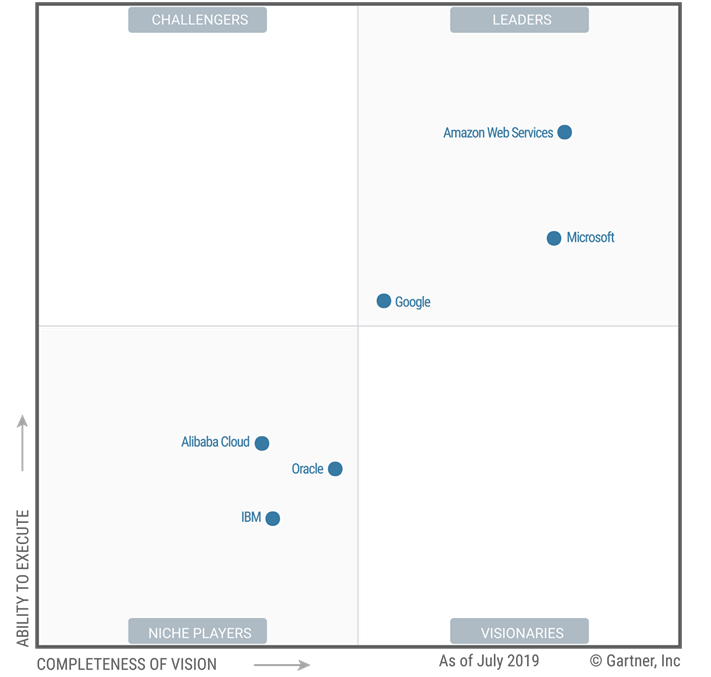
\includegraphics[width=0.9\textwidth]{figures/CloudIaaS.png}
\caption{Gartner (07/2019) pilvipalveluiden vertailu. \citep{top_cloud}}\label{gartner}
\end{figure}

\chapter{Palvelun laatu\label{laatu}}
Palvelutoiminnassa tuotannon laatu on kriittinen tekijä. Palvelun tuottaja on velvollinen tarjoamaan sovittua laatutasoa palveluistaan. Palveluiden laatu on myös tarjouspyynnöissä ja kilpailutuksessa tärkeä valintatekijä. Konesalipalveluille ja pilvipalveluille on asetettu maailmanlaajuisten standardien kautta laatukriteerit, jotka niiden tulee täyttää. Pääsääntöisesti kaikki palvelutarjoavat täyttävät nämä ISO standardin mukaiset laatukriteerit. Laadun mittaamisella osoitetaan avoimesti asiakkaille kuukausittain ja vuosittainen laatutaso, johon on vertailujaksolla päästy. Nämä mittaamismenetelmät ovat vakiintuneita käytäntöjä IT-palvelutoimittajien parissa. Standardit edellyttävät kolmannen osapuolen säännölliset tarkastukset, jotta sertifiointi pysyy voimassa.
\section{Laatuvaatimukset}
Organisaation laadunhallintajärjestelmien kansainvälinen standardi on ISO 9001. Standardiin sitoutumalla palveluntarjoaja osoittaa tuotteen ja palvelun laadun olevan asiakkaan odotusten mukainen. Asiakastyytyväisyyttä mitataan ja ylläpidetään laadunhallintajärjestelmien avulla. Standardin mukaisesti palveluntarjoajan laadunhallintajärjestelmän politiikka ja strategia ovat osa organisaation liiketoimintastrategiaa. Standardia voidaan soveltaa kaikentyyppisiin yrityksiin kaikilla toimialoilla. Standardi edistää riskiperusteista lähestymistapaa, jossa korostetaan ennaltaehkäisevien toimenpiteiden suunnittelua. Kaikki suurimmat konesalipalvelut ja pilvipalvelut ovat ISO 9001 sertifioituja \citep{borenstein2011cloud} \citep{iso9001}.

Tunnetuin tietoturvallisuuden hallintajärjestelmien kansainvälinen standardi on ISO/IEC 27001. Sen avulla palveluntarjoaja kykenee laatimaan tieturvan hallintapolitiikan ja –tavoitteet. Standardi tarjoaa viitekehyksen hallita organisaation velvollisuuksia noudattaa oikeudellisia vaatimuksia, jotka koskettaa konesalipalveluja ja pilvipalveluja. Standardin avulla palveluntarjoaja voi osoittaa, että järjestelmiin tallennetut tiedot ovat vain niiden henkilöiden saatavissa, joilla on niihin oikeus. Lisäksi tietojen eheys turvaa tietojen ja käsittelymenetelmien oikeellisuuden ja täydellisyyden. Palvelutarjoajan tekninen suojaus kattaa tietolaitepetokset. Kaikki suurimmat konesalipalvelut ja pilvipalvelut ovat ISO 27001 standardin mukaisia \citep{pattern} \citep{iso27001}.

Ympäristöstandardi ISO 14001 tarkastelee koko yrityksen toimintaa sisältäen ympäristösuojelun, kasvihuonekaasupäästöjen hallinnan ja ilmastomuutokseen sopeutumisen. Palvelutarjoaja sitoutuu standardin puitteissa varmistamaan ympäristöasioiden jatkuvan kehittämisen. Palvelutarjoajat haluavat osoittaa, että he ovat mukana vastuullisessa ympäristöjärjestelmien kehittämisessä. Suurin osa konesalipalvelujen ja pilvipalvelujen tarjoajista on mukana ISO 14001 standardissa \citep{iso14000}.
\section{Laadun mittaaminen}
Ohjelmistotuotannon palvelun laadun mittaaminen pohjautuu ISO 25000 standardiin, joka tunnetaan myös nimellä (System and Software Quality Requirements and Evaluation) SQuaRE. Standardi asettaa viitekehityksen ohjelmistotuotannon laadun mittaamiseen \citep{iso25000}. Standardin ISO 25010 mukaisesti hyvä tapa on jakaa tuotteen laatu eri ominaisuuksiin \citep{iso25010}. Näiden standardien pohjalta Quality Model of Cloud Service julkaisussa ehdotetaan pilvipalveluiden mittaamista kuudella kriteerillä: käytettävyys (\emph{usability}), turvallisuus (\emph{security}), luotettavuus (\emph{reliability}), konkreettisuus (\emph{tangibility}), reagointikyky (\emph{responsiveness}) ja empatia (\emph{empathy}) \citep{qualitymodel}.

Käytettävyys (\emph{usability}) tarkoittaa pilvipalveluissa, että asiakkaalla on mahdollisuus itsenäisesti tilata ja käyttää palveluja. Tärkeintä asiakkaalle on, että pilvipalvelun käyttö on helppoa, tehokasta ja nautittavaa \citep{adaptive}. Nämä kriteerit saadaan täytettyä hyvillä ohjeilla, helppokäyttöisellä käyttöliittymällä ja selkokielisillä virheilmoituksilla. Näin saadaan asiakkaalle subjektiivinen tuntemus käytettävyydeltään hyvästä pilvipalvelusta \citep{qualitymodel}.

Turvallisuus (\emph{security}) on tärkeä palvelukriteeri kaikille pilvipalveluille. Keskitettyjen palveluiden haasteena on rakentaa riittävän turvallinen palvelu asiakkaille. Pilvipalveluiden tulee tarjota asiakkaille toimintaympäristö, jossa tietojen luottamuksellisuus ja eheys sekä asiakkaiden yksityisyyden suoja on tarkkaan huomioitu. Pilvipalvelujen tarjoajan tulee myös huolehtia jäljitettävyydestä, jossa palveluprosessin toiminnot tallennetaan ja ne tulee voida jäljittää jälkikäteen \citep{qualitymodel}.

Luotettavuus (\emph{reliability}) on olennainen ominaisuus pilvipalvelulle. Asiakkaalle tärkeitä ominaisuuksia on palvelun saatavuus ja jatkuvuus. Asiakkaat odottavat, ettei pilvipalvelussa ole laitteisto-ongelmia, ohjelmistovikoja tai muita vikoja, jotka voidaan aiheuttaa ongelmia palvelun saatavuuteen. Luotettavuuden kriteerejä ovat saatavuus (availability), täydellisyys (completeness), oikeudenmukaisuus (correctness), jatkuvuus (continuity) ja vakaus (stability). Asiakkaiden vaatimuksena on, että palvelu on ympärivuorokautisesti saavutettavissa ilman katkoja \citep{qualitymodel}.

Konkreettisuus (\emph{tangibility}) on pilvipalvelun tarjoajan mittari avoimuudelle. Palveluntarjoajan tulee antaa asiakkaalle näkyvyyttä palvelun laatutasoon raporttien muodossa. Lisäksi palveluntarjoajan tulee toimia ammattimaisesti niin, että kehitystoimenpiteet perustuvat asianmukaisiin taitoihin ja asiantuntemukseen. Tämä käyttäjäkokemus on mahdollista tarjota asiakkaalle hyvän käyttöliittymän kautta \citep{qualitymodel}.

Reagointikyky (\emph{responsiveness}) tarkoittaa tietojenkäsittelyssä järjestelmän tai toiminnallisen yksikön kykyä suorittaa sille osoitetut tehtävät tietyssä ajassa \citep{dictionary}. Pilvipalvelutarjoajan tulee olla valmis ja kykenevä auttamaan asiakkaita tarjoamalla nopeaa ja oikea-aikaista palvelua. Reagointikyvyn ominaisuuksia ovat ajantasaisuus, vuorovaikutus sekä kyky toimittaa resursseja asiakkaan tarpeiden mukaisesti \citep{qualitymodel}.

Empatia (\emph{empathy}) tarkoitetaan, että pilvipalvelun tarjoaja on kykenevä muokkaamaan palveluaan yksittäisten asiakkaiden tarpeiden mukaisesti. Asiakaskokemus syntyy kokemuksien mukaan. Pilvipalveluntarjoajan tulisi kattaa asiakkaan vaatimukset ja tarjota asiakkaalle laadukasta palvelua. Palvelutarjoaja voi saavuttaa nämä ominaisuudet panostamalla itsepalveluun, palveluiden mitattavuuteen ja aloitekykyyn. Palveluntarjoajan tulisi olla proaktiivinen ja tunnistaa asiakkaan vaatimukset sekä ehdottaa muutoksia tarpeiden mukaisesti \citep{qualitymodel}.

\chapter{Palveluiden vertailu\label{vertailu}}

\section{Taustatiedot}
Pilvipalvelujen ja konesalipalveluiden laatua verrattiin tutkielmassa keräämällä aineisto, joka sisälsi raportoidut tiketit eri palvelutoimittajien järjestelmiin. Tutkielmassa tarkasteltiin erikseen palveluongelmia (\emph{incident}) ja palvelupyyntöjä (\emph{service request}). Molemmista palveluista oli saatavissa tutkielmaa varten kattavat tilastot tiketeistä. Lisäksi tutkielmaa varten haastateltiin Finnairin työntekijöitä ja pyydettiin heitä kokemuksia pilvi- ja konesalipalveluista. Näin saatiin myös subjektiivinen näkökulma tutkielmaan.

Isot, laaja-alaiset ja vakavat ongelmatilanteet luokitellaan termillä \emph{Major Incident}. Tässä tilanteessa virhetilanteesta lähetetään sähköpostitse tiedote yhtiön sisäisesti eri sidosryhmille ja ongelmatilanteen selvitykseen nimitetään oma asiantuntija. Nämä vakavat ongelmatilanteet on erikseen tilastoitu ja niistä tehdään myös jälkikäteen erillinen selvitys syistä. Vakavat ongelmat voivat olla haitaksi lentoliikenteelle ja sitä kautta myös Finnairin ydinliiketoiminnalle. Näitä vakavia virhetilanteita tulisi välttää kaikin keinoin ja niistä tulisi toipua mahdollisimman nopeasti. Tutkielmassa perehdyttiin näiden vakavien virheiden määrään ja vakavuusluokitukseen.
\section{Laatuvertailut}
Tutkielmassa verrattiin konesalipalvelun aikaisia tikettejä sekä pilvipalveista raportoituja tikettejä. Vertailua tehtiin erikseen virhetilanteista ja palvelupyynnöistä. Tutkielmassa tarkasteltiin tikettien määrää sekä tikettien tärkeysastetta (\emph{priority}). Palvelupyyntöjen osalta tarkasteltiin myös tikettien ratkaisuaikoja, koska se vaikuttaa palvelukokemukseen.

Tiketit on luokiteltu viisiportaisella asteikolla eri tärkeysasteille. Samaa luokittelua on käytetty konesalipalveluissa ja pilvipalveluissa, joten tilastot ovat vertailukelpoisia.  Luokittelu perustuu virhetilanteen kriittisyyteen ja virhetilanteen vaikutukseen tuotantoon. P1 tason tiketin aukaistaan tilanteessa, jossa ohjelmalla on kriittinen yrityksen tuotannolle ja kyseisellä virhetilanteella on iso laaja-alainen vaikutus. Osa virhetilanteista on automaattitikettejä, jotka valvontalaitteisto aukaisee automaattisesti. Muut tiketit ovat käsin aukaistuja tikettejä niin, että loppukäyttäjä raportoi ongelmasta IT toimittajan asiakaspalveluun. 

Pilvipalveluissa tarkasteltava aikajakso on 1.1.--30.9.2021. Tänä aikana virhetilanneisiin liittyviä käsin avattuja kriittisiä tikettejä on ollut yhteensä 22 ja vähemmän kriittisiä tikettejä 194. Kuvassa \ref{fig:pilvitiketit} nähdään tikettien määrät vuoden 2021 eri kuukausina sekä jakautuma kriittisten ja vähemmän kriittisten tikettien välillä. Kuvasta voidaan todeta, että kriittisiä virhetilanteita on ollut vähäinen määrä kuukausittain. Pääasiassa virhetilanteet ovat olleet vähemmän kriittisiä. Kuvasta nähdään, että kriittisiä virhetilanteiden määrässä ei ole ollut kuukausittain isoa vaihtelua. Taulukosta \ref{table:automaatti} nähdään kuinka paljon eri tärkeysasteen tikettejä on ollut vuoden 2021 aikana ja miten tiketit on jakautuneet käsin tehtyjen ja automaattitikettien välikkä. Taulukosta voidaan todeta, että kriittisiä automaattitikettejä on ollut vähän verrattuna kokonaismäärään. Taulukosta nähdään, että käsin on avattu pääasiassa P3 tason tikettejä, jotka ovat vähemmän kriittisiä.

\begin{filecontents}{data1.dat}
X Time  	Part1  Part2
1 tammi  	2	22
2 helmi		1	25
3 maalis	2	18
4 huhti		3	41
5 touko		2	28
6 kesä		2	13
7 heinä		2	14
8 elo       3   15
9 syys      5   18
\end{filecontents}

\begin{figure}[ht]
\begin{tikzpicture}
\begin{axis}[
axis lines=middle,
ymin=0,
legend pos=outer north east,nodes near coords,
x label style={at={(current axis.right of origin)},anchor=north, below=10mm},
title={\textbf{\textit{}}},
    xlabel=Vuosi 2021,
    ylabel=Määrä,
    xticklabel style = {rotate=30,anchor=east},
    enlargelimits = false,
    xticklabels from table={data1.dat}{Time},xtick=data]
\addplot[blue,thick,mark=square*] table [y=Part1,x=X]{data1.dat};
\addlegendentry{P1+P2 tiketit}
\addplot[red,thick,mark=square*] table [y= Part2,x=X]{data1.dat};
\addlegendentry{Muut tiketit}
\end{axis}
\end{tikzpicture}
\caption{Vertailu käsin avattujen kriittisten ja vähemmän kriittisten tikettien välillä pilvipalveluissa}
\label{fig:pilvitiketit}
\end{figure}

\begin{table}[ht]
\centering
\begin{tabular}{||c c c||} 
 \hline
 Kriittisyys & Käsin avatut tiketit & Automaattitiketit \\ [0.5ex] 
 \hline\hline
 P1 & 5 & 14 \\ 
 P2 & 19 & 0 \\
 P3 & 173 & 17 \\
 P4 & 9 & 1 \\
 P5 & 9 & 348 \\
 \textbf{Yhteensä} & \textbf{215} & \textbf{380}\\ [1ex] 
 \hline
\end{tabular}
\caption{Pilvipalveluissa avattut tiketit vuonna 2021}
\label{table:automaatti}
\end{table}

Pilvipalveluissa oli aikajaksolla 1.1.--30.9.2021 yhteensä 224 palvelupyyntöä. Palvelupyyntöjen ratkaisuaika oli keskimäärin 244 tuntia eli reilu 10 päivää. Maksimiarvo ratkaisuajalla oli 2213 tuntia eli yli 92 päivää. Kuvassa \ref{fig:pilvipyynto} nähdään palvelupyyntötikettien määrät vuoden 2021 eri kuukausina. Kuvasta voidaan todeta, että palvelupyyntöjen määrä on ollut nousussa. Nousu johtuu siitä, että pilvipalvelujen käyttöönotto on edelleen kesken ja muutoksia ympäristöön tehdään jatkuvasti Lisäksi Finnairin ydinliiketoiminta on elpymässä ja liiketoiminnan kehitys on alettu tekemään korona-ajan jälkeen.

\begin{filecontents}{data2.dat}
X Time  	Part1
1 tammi  	8
2 helmi		21
3 maalis	21
4 huhti		16
5 touko		38
6 kesä		34
7 heinä		23
8 elo       31
9 syys      32
\end{filecontents}

\begin{figure}[ht]
\begin{tikzpicture}
\begin{axis}[
axis lines=middle,
ymin=0,
legend pos=south east,nodes near coords,
x label style={at={(current axis.right of origin)},anchor=north, below=10mm},
title={\textbf{\textit{}}},
    xlabel=Vuosi 2021,
    ylabel=Määrä,
    xticklabel style = {rotate=30,anchor=east},
    enlargelimits = false,
    xticklabels from table={data2.dat}{Time},xtick=data]
\addplot[blue,thick,mark=square*] table [y=Part1,x=X]{data2.dat};
\addlegendentry{Palvelupyynnöt}
\end{axis}
\end{tikzpicture}
\caption{Tilasto palvelupyynnöistä pilvipalveluissa}
\label{fig:pilvipyynto}
\end{figure}

\section{Haastattelut}
Haastatteluissa selvitettiin minkälainen subjektiivinen käsitys Finnair IT asiantuntijalla ja johtajalla on tuotannon laadusta, kun verrataan pilvipalvelua ja konesalipalvelua. Haastatteluun osallistuneilla henkilöillä on kokemusta molemmista toimintamalleista. Haastatteluissa haettiin heidän henkilökohtaisia mielipiteitä aiheesta ja mielipiteiden ei tarvinnut perustua todellisiin faktatietoihin. Faktatietoihin perustuva vertailua tehtiin tämän tutkimuksen muissa osissa. Subjektiivinen näkökulma on tärkeä selvittää, koska laatu perustuu myös tuntemukseen siitä kuinka hyvin asiakasta palvellaan sekä minkälainen olo hänelle on toiminnasta. Haastattelu jakautui kahteen osaan. Ensimmäisessä osassa selvitettiin tuotannon laatua virhetilanteiden (\emph{incident}) kautta ja toisessa osassa palvelupyyntöjen (\emph{service request}) kautta.

Haastattelussa todettiin, että tuotanto on pilvipalvelujen kautta ollut jonkin verran stabiilimpaa. IT asiantuntija korosti, että laadun ero pilvipalvelujen ja konesalinpalvelujen välillä ei ole ollut iso, mutta eron on silti huomannut. Pilvipalveluissa on ollut vähemmän infrastruktuuriin liittyviä ongelmia, kuten verkkoliikenteen ongelmat. Silti pilvipalveluissa on havaittu myös perinteisiä palvelimiin liittyviä ongelmia, kuten muistitilan ja levytilan loppuminen. Pilvipalveluissa ongelmien sattuessa vaikutukset ovat olleet suuremmat ja laajemmat. Tosin pilvipalveluissa näitä laajempia ongelmia on harvemmin sattunut, kun tilannetta verrataan konesalipalveluihin.

IT johtajan kiinnitti huomiota, että nykyinen pilviympäristö on vasta alle vuoden vanha ja kaikkia kokemuksia ei ole vielä saatu. Virhetilanteita on hänen mukaansa ollut vähemmän ja ne on ollut lyhytkestoisempia kuin aikaisemmin konesalipalveluiden kanssa. Nykyisessä AWS pilvipalvelussa tuotanto on hajautettu useammalle käyttöalueelle (\emph{AWS Zone}). Tällöin yhden käyttöalueen ongelmat eivät heijastu koko Finnairin tuotantoon. Tämä on auttanut siihen, että virhetilanteita on ollut vähemmän kuin konesalipalvelussa, jossa tuotanto toteutettiin yhdestä fyysisestä paikasta. Yhdessä konesalissa tapahtuva virhe heijastui laajasti koko tuotantoon. IT johtaja painotti, että tilanne tulee entisestään paranemaan pilvipalveluiden osalta, koska pilvipalveluiden toimittaja ja asiakkaan tulee molempien kehittää jatkuvasti ympäristöä eikä korjausvelkaa synny niin paljon kuin konesalipalveluissa.

Vakavia virhetilanteita asiantuntijan mukaan ollut nyt vähemmän, mutta jos verrataan tilannetta pidemmällä aikajaksolla, niin vakavia ongelmia on ollut suunnilleen sama määrä. Vakavien virhetilanteiden määrä on asiantuntijan mukaan riippuvainen kuinka paljon tehdään muutoksia ympäristöön. Jos tehdä isoja laajoja muutoksia IT ympäristöön, niin se sisältää aina riskejä, jotka voivat realisoitua vakavina ongelmina ja toimintahäiriöinä. Yrityksen pilvipalveluympäristö on sen verran uusi, ettei vielä ole tarvinnut tehdä isompia muutoksia ympäristöön, jolloin myös vakavia ongelmia ei ole syntynyt. Konesalipalveluissa on riski, että yksittäisen työntekijän tekemä inhimillinen virhe voi aiheuttaa isoja ongelmia. IT johtajan mukaan vakavia virhetilanteita on ollut pilvipalveluissa vähemmän eivätkä ongelmat ole olleet niin pitkäkestoisia. Tämä on näkynyt parempana tuotannon laatuna pilvipalveluissa ja parantanut Finnair IT palvelujen käytettävyyttä.

Asiantuntija mukaan ongelmien ratkaisunopeudessa ei ole ollut suurta ero kun verrataan pilvipalveluja ja konesalipalveluja. Konesalipalveluissa koko ympäristön hallinta oli keskitetty yhdelle yritykselle, jonka vastuulla oli kokonaisvaltaisesti pitää huolta, että palvelut toimivat. Ongelma tilanteiden selvitys oli tässä tilanteessa suoraviivaisempaa, koska vastuu yrityksiä oli vain yksi. Isolla konesalipalvelun tarjoajalla oli myös iso määrä eri alan asiantuntijoita valmiina selvittämään ongelmatilanteita. Tämä vaikutti ratkaisunopeuteen, kun oikeat asiantuntijat saatiin välittömästi mukaan selvitystyöhön. Pilvipalveluissa vastuut on hajautettu eri toimijoille sekä osa vastuista on otettu Finnairin hoidettavaksi. Tämä vaikuttaa ongelmien ratkaisunopeuteen, kun vastuualueet ovat epäselviä ja useampi toimittaja yrittää ratkaista ongelmaa. Finnairin asiantuntijan mukaan pilvipalveluissa on ongelmien ratkaiseminen ollut hitaampaa näistä syistä. Toisaalta yksinkertaisemmat ja pienemmät ongelmat ratkaistaan pilvipalveluissa nopeammin, kun ympäristö on topologialtaan selkeämpi.

IT johtaja oli samaa mieltä, että ongelmatilanteiden ratkaiseminen on ollut pilvipalveluissa nopeampaa kuin konesalipalveluissa. Pitää kuitenkin muistaa, että myös pilvipalveluissa voidaan tehdä isoja virheitä. Näistä ongelmista on kuitenkin pilvipalveluissa parempi näkyvyys, koska tiedot ovat julkisia. Konesalipalvelut ovat suljettuja ja niissä esiintyvät ongelmat toimittajan on mahdollista peittää. Konesalipalveluiden toimittaja voi kertoa vain niistä ongelmista, jotka ovat näkyneet asiakkaille. Pilvipalveluissa on ulkoisia tilannesivuja Internetissä, joissa näkyy ongelmatilanteet ja niihin tehdyt ratkaisut.

Kun verrataan pilvipalveluja ja konesalipalveluja palvelupyyntöjen (\emph{service request}) näkökulmasta, niin Finnairin asiantuntijan mukaan palveluissa ei ollut merkittävää eroa. Uuden pilvipalvelutoimittaan palvelualttius on ollut parempaa ja reagointi nopeampaa, mutta tähän voi vaikuttaa myös että uusi toimittaja haluaa näyttää asiakkaalle alkuun hyvää ja huolellista palvelua. Konesalipalvelut, jotka olivat keskitettyjä, toiminta ei ollut niin ketterää. Pilvipalvelut toimitetaan enemmän ketterien menetelmien mukaisesti, jolloin toiminta on joustavampaa. Konesalipalveluissa yksittäisen palvelupyynnön tekemiseen kului enemmän aikaa, koska jossain tapauksissa muutos haluttiin projektoida ja tämä loi lisää hidastavaa byrokratiaa. Pilvipalveluissa esimerkiksi uusien palvelimien lisääminen ympäristöön on hyvin suoraviivaista ja nopeaa. Näissä tilanteissa palvelupyyntöjen toteutus on nopeaa. Konesalipalveluissa palvelimien poisto palvelusta ei ole suoraviivaista. Palvelimesta ei voida pelkästään katkaista sähkövirta, vaan sille tulee tehdä myös muita poistotoimenpiteitä, joista tulee ylimääräisiä kustannuksia. Pilvipalveluissa taas palvelimien poisto on yksinkertaista ja nopeaa. Poisto voidaan tehdä konekielisesti yhdellä komennolla ja siitä syntyvät taloudelliset säästöt ovat välittömästi saatavissa.

IT johtajan mukaan pilvipalvelut ovat ketteriä ja nopean reagoinnin palvelupyyntöihin. Konesalipalveluissa tarvitaan enemmän työtä ja byrokratiaa pieniinkin muutoksiin. Pilvipalvelut ovat vakioituja automaattisia prosesseja, jotka mahdollistavat nopean toiminnan. Automatisoidut prosessit antavat myös enemmän ketteryyttä ja ovat varmempia laadultaan. Inhimillisten virheiden määrä on pienempi, kun prosessit hoidetaan automatisoidusti. Tämä antaa myös enemmän mahdollisuuksia ja joustoa asiakkaalle. IT johtaja piti tärkeänä, että pilvipalveluissa kiinnitetään huomiota tietoturvaan. Pilvipalvelut ovat liiankin joustavia, jolloin tietoturva unohtuu helposti, jollei siihen erityisesti kiinnitetä huomiota. Kaikki tietoturvaratkaisu eivät ole automatisoituja. Kaiken kaikkiaan pilvipalveluiden ylläpito on hänen mukaan haastavampaa ja vaatii yhtenäisen toimintatavan asiakkaalla. Pilvipalveluiden toimittaja ei pakota asiakasta tiettyihin toimintatapoihin. Myös IT arkkitehtuurin näkökulmasta pilvipalvelut korruptoituvat helpommin verrattuna konesalipalveluihin. IT johtaja tarkoitti korruptoitumisella sitä, että ympäristön monimutkaisuus tulee jossain vaiheessa vastaan, kun tehdään jatkuvaa kehitystä. Jossain vaiheessa pilviympäristö tulee muokata uudelleen, jollei arkkitehtuuri asioista pidetä riittävästi huolta muutostilanteissa.  

Tutkielman haastattelussa kysyttiin myös haastateltavilta yleisnäkemystä, siitä kumpi toimintamalli on parempi Finnairille, kun verrataan konesalipalveluja ja pilvipalveluja. Asiantuntija piti pilvipalveluja oikeana suuntana toiminnan parantamiseen. Asiantuntija painotti, että pilvipalvelut ovat huomattavasti joustavammat ja sitä kautta taloudellisten säästöjen tekeminen on nopeampaa sekä helpompaa. Pilvipalveluissa toimintaympäristö voidaan muokata itsenäisesti ilman isompaa byrokratiaa. Pilvipalveluihin siirtyminen oli väistämätön aihe ja se olisi tullut tehdä jossain vaiheessa. Asiantuntijan mukaan nyt oli hyvä aika tehdä muutostyö, kun koronaviruksen takia Finnairin toiminta oli hiljaisempaa. Finnair asiantuntija painotti, että pilvipalveluihin siirto on vielä kesken, siksi kaikkia hyötyjä ja haittoja ei ole vielä koettu. Tulevaisuus ei ole hänen mukaan niin selvä ja pilvipalvelujen toimintamallissa voi tulla myös yllätyksiä tulevaisuudessa. Kokonaisarvosanan (asteikolla 0-5) asiantuntija antoi konesaliyrityksen X palvelusta arvosanan 4- ja AWS pilvipalveluille arvosanan 4.

IT johtaja piti haastattelussa pilvipalveluja oikeana ratkaisuna Finnairin kannalta. Yrityksen tulee myös laajemmin muuttua toimintatavoiltaan ketterämmäksi. Tilanteet muuttuvat nykymaailmassa nopeasti ja muutoksiin tulee reagoida välittömästi. Pilvipalvelut ovatkin yrityksen strategian mukainen valinta. Pilvipalvelut antavat enemmän mahdollisuuksia kuin konesalipalvelut. IT johtaja muistutti, että pilvipalvelut vaativat enemmän teknistä osaamista myös asiakkaalta eikä palveluja voida enää ostaa niin helposti kuin konesalipalveluissa. Yrityksellä X oli tarjota konesalipalveluiden yhdessä lukuisia IT alan asiantuntijoita auttamaan ratkaisujen rakentamisessa. Tätä mahdollisuutta ei enää ole pilvipalveluiden kanssa, vaan asiakkaan tulee olla myös itse aktiivinen kun muutoksia tehdään. Pilvipalveluja tuleekin kehittää fiksusti huomioiden arkkitehtuuriset ratkaisut ja tietoturva. Kokonaisarvosanaksi (asteikolla 0-5) IT johtaja antoi konesaliyritykselle X palveluista 3 ja AWS pilvipalvelulle 4. IT johtaja painotti, että AWS arvosanaa on mahdollista edelleen nostaa, kun Finnairin omia IT prosesseja saadaan edelleen kehitettyä ja opitaan toimimaan pilvipalveluiden kanssa. Yrityksen historia painottuu pitkältä ajalta konesalipalveluihin ja muutostyö vielä aikaa. Vasta myöhemmin AWS palveluiden arvosana voi nousta.  
\chapter{Analyysi\label{analyysi}}
Tutkimuksessa verrattiin konesalipalvelun ja pilvipalvelun laatua raportoitujen tikettien perusteella sekä IT henkilön haastatteluiden pohjalta. Tutkimuksen tuloksista laadittiin analyysi, jossa vastataan tutkimuskysymykseen, kumpi palvelumalleista on laadultaan parempi. Tutkimuksen tavoitteena oli myös selvittää tekikö Finnair strategisesti oikean ratkaisun siirtyessään täysimääräisesti pilvipalveluiden käyttäjäksi.

Tikettitilastoja verrattaessa huomataan, että konesalipalveluissa on ollut enemmän kriittisiä tikettejä kuin pilvipalveluissa.  Pilvipalveluissa vuoden 2021 aikana kriittisiä tikettejä on kuukausittain ollut vain muutamia kappaleita. Verrattaessa virhetilanteista aukaistujen tikettien kokonaismäärää huomataan, että tikettejä on lähes yhtä paljon kuukausittain pilvipalveluissa ja konesalipalveluissa. Konesalipalveluista ei ollut tutkimukseen saatavissa automaattitikettien tilastoja, joten analyysiä automaattitikettien osalta ei voida tutkimuksessa tehdä. Tuloksien perusteella voidaan todeta, että tikettimäärä on molemmissa palvelumalleissa ollut lähes sama, mutta pilvipalveluissa kriittisiä virheitä on ollut vähemmän. Tutkimuksen analyysinä voidaan todeta, että pilvipalveluiden laatu on ollut parempi tarkastellulla aikajaksolla.

Tutkimuksessa verrattiin palvelumalleja myös palvelupyyntötikettien perusteella. Tuloksista voidaan todeta, että palvelupyyntöjä on tehty yhtä paljon konesalipalveluissa ja pilvipalveluissa. Pilvipalveluissa palvelupyyntöjen ratkaisuaika on ollut keskimäärin reilu 10 päivää ja konesalipalveluissa keskimääräin 2,5 päivää. Konesalipalveluissa palvelupyynnöt on ratkaisu nopeammin. Konesalipalveluissa maksimiarvo ratkaisuajalla on ollut alhaisempi kuin pilvipalveluissa. Tuloksien perusteella voidaan todeta, että konesalipalveluissa palvelupyyntöjen ratkaisunopeus on ollut nopeampi ja sen osalta laatu ollut parempaa käyttäjille.

Haastatteluissa IT asiantuntija ja IT johtaja toivat esiin erilaisia näkökulmia verrattaessa konepalveluja pilvipalveluja. Haastattelujen perusteella voidaan todeta, että tuotanto on pilvipalvelujen kautta ollut jonkin verran stabiilimpaa, mutta laadun ero pilvipalvelujen ja konesalinpalvelujen välillä ei ole ollut iso. Pilvipalveluissa on ollut vähemmän infrastruktuuriin liittyviä ongelmia kuin konesalipalveluissa. Pilvipalveluissa ongelmien sattuessa vaikutukset ovat olleet suuremmat ja laajemmat. Tosin pilvipalveluissa laajempia ongelmia on harvemmin sattunut. Haastatteluiden perusteella virhetilanteita on pilvipalveluissa ollut vähemmän ja virhetilanteet ovat olleet lyhytkestoisempia kuin aikaisemmin konesalipalveluiden kanssa. Ongelmatilanteet on ratkaistu pilvipalveluissa nopeammin.

Kun verrataan pilvipalveluja ja konesalipalveluja palvelupyyntöjen näkökulmasta, niin palveluissa ei ole ollut merkittävää eroa haastattelujen perusteella. Pilvipalvelut ovat ketteriä ja mahdollistavat nopean reagoinnin palvelupyyntöihin. Konesalipalveluissa tarvitaan enemmän työtä ja byrokratiaa pieniinkin muutoksiin. Pilvipalvelut ovat vakioituja automaattisia prosesseja, jotka mahdollistavat nopean toiminnan, mutta toisaalta pilvipalveluiden ylläpito on haastavampaa ja vaatii yhtenäisen toimintatavan asiakkaalta. Toisaalta pilvipalvelut ovat liiankin joustavia ja tietoturvaan tulee erityisesti kiinnittää huomiota.

Tutkimuksen haastatteluissa kysyttiin haastateltavilta yleisnäkemystä, siitä kumpi toimintamalli on parempi Finnairille, kun verrataan konesalipalveluja ja pilvipalveluja.  Pilvipalveluja pidettiin oikeana suuntana toiminnan parantamiseen. Pilvipalvelut pidettiin joustavampana ja sitä kautta taloudellisten säästöjen tekeminen on nopeampaa. Pilvipalvelut ovat Finnairin strategian mukainen valinta, koska pilvipalvelut antavat enemmän mahdollisuuksia kuin konesalipalvelu. Finnairin tulee myös laajemmin muuttua toimintatavoiltaan ketterämmäksi.

Tutkimuksen tuloksista voidaan todeta, että pilvipalvelut ovat oikea ratkaisu Finnairin kannalta. Pilvipalveluihin siirto on vielä kesken, siksi kaikkia hyötyjä ja haittoja ei ole vielä havaittu. Virhetilanteista raportoituen tikettien perusteella pilvipalveluissa laatu on ollut parempaa ja vakavia häiriötilanteita on ollut vähemmän. Konesalipalveluissa palvelupyyntöjen ratkaisunopeus oli nopeampi ja sen osalta laatu oli parempaa käyttäjille. Haastatteluissa pilvipalveluja pidettiin joustavampana ja asiantuntijat pitivät tärkeänä, että muutoksiin voidaan reagoida nopeasti. Haastatteluissa pilvipalveluille annettiin parempi kokonaisarvosana. 



\chapter{Yhteenveto\label{conclusions}}
Tutkimuksen kohteena oli Finnair Oyj:n konesalipalveluiden ulkoistus pilvipalveluun ja sen laadun vertailu edeltäneeseen ratkaisuun, jossa palvelu tuotettiin perinteisenä konesalipalveluna. Finnair Oyj:ssa palvelemien ylläpidon kehityspolku on edennyt vuosikymmenien aikana omista palvelimista vuonna 2020 käyttöön otettuihin pilvipalveluihin. Vuoden 2021 aikana Finnairilla on sisäisesti keskustelu pilvipalveluiden laadusta, mutta varsinaista yhteenvetoa ei ole tehty palvelun laadusta. Tutkimuksen tavoitteena oli verrata konesalipalveluiden ja pilvipalveluiden laatua. Tutkimuksen ulkopuolelle jätettiin palvelumallien kustannuksen vertailu. Tutkimuskysymyksenä oli selvittää tekikö Finnair oikean ratkaisun siirtyessään laajamittaisesti pilvipalveluihin ja onko pilvipalveluiden laatu parempaa kuin perinteiden konesalipalveluiden laatu.

Tutkimuksessa taustatietona selvitettiin erilaisia palvelumalleja, joilla konesalipalveluja tuotetaan asiakkaille. Tutkimuksessa perehdyttiin näiden palvelukuvauksiin sisältöihin ja arviointiin erilaisia malleja, millä palvelimien hallinnointia voidaan tarjota asiakkaille. Tutkimuksessa selvitettiin pilvipalveluiden markkinoita ja verrattiin suurempia palvelutarjoavia. Tutkimuksessa perehdyttiin myös IT palveluiden laadun mittaamiseen ja minkälaisia laatuvaatimuksia asetetaan palvelimien ylläpidolle.

Finnairille konesalipalveluita tuotti aikaisemmin yritys X, jonka virallinen nimeä ei käytetty tutkimuksessa yrityssalaisuuksien takia. Tutkimuksessa kerättiin tilastotiedot konesalipalveluiden virhetilanteiden tiketeistä sekä palvelupyynnöistä, joita oli laadittu konesaliympäristön muutoksista. Näitä tilastotietoja verrattiin vastaaviin tietoihin nykyisestä pilvipalvelusta. Tutkimukseen kuului myös kaksi haastattelua, joissa selvitettiin Finnairin IT asiantuntijan ja IT johtajan subjektiiviset mielipiteet palveluiden laadusta konesalipalveluissa ja pilvipalveluissa.

Tutkimuksesta laadittiin analyysi ja yhteenveto. Tutkimuksessa havaittiin, että pilvipalveluihin siirto on vielä kesken, joten laadusta ei ole vielä kokonaiskuvaa. Tutkimuksen perusteella voidaan todeta, että pilvipalveluiden laatu on ollut parempaa ja vakavia häiriötilanteita on ollut vähemmän. Konesalipalveluissa oli enemmän kriittisiä tikettejä kuin pilvipalveluissa. Tutkimuksessa verrattiin myös palvelupyyntötikettejä. Pilvipalveluissa palvelupyyntöjä on ratkaisu hitaammin ja konesalipalveluissa palvelukokemus oli käyttäjille parempi. Haastatteluissa pilvipalveluja pidettiin vakaampana ja ketterämpänä, mikä mahdollistaa nopeamman reagoinnin muutospyyntöihin. Toisaalta ketteryys vaatii myös asiakkaalta tarkkuutta ja hyviä sisäisiä prosesseja. Tutkimuksen haastatteluissa tietoturvaa pidettiin isompana riskinä pilvipalveluissa, koska kaikki tietoturvaratkaisut eivät ole automatisoituja prosesseja.

Tutkimuksessa todettiin, että pilvipalvelut ovat oikea ratkaisu Finnairille ja yrityksen strategian mukainen suunta kohti ketterämpiä toimintamalleja. Pilvipalveluiden siirto on vielä kesken ja tilastoja tulee tarkastella myöhemmin uudestaan. Pilvipalveluissa laatu on ollut parempaa ja vakavia virhetilanteita on ollut vähemmän. Kokonaisuutena häiriötilanteista tikettejä on raportoitu yhtä paljon molemmissa malleissa. Konesalipalveluissa palvelupyyntöjen ratkaisuajat olivat lyhyempiä ja käyttäjäkokemusta sitä kautta parempi. Haastatteluissa pilvipalveluiden vahvuutena pidettiin joustavuutta ja nopeaa reagointia muutoksiin. Pilvipalvelulle annettiin tutkimuksen haastatteluissa parempi arvosana palvelun laadusta.

%%%%%%%%%%%%%%%%%%%%%%%%%%%%%%%%%%%%%%%%%%%%%%%%%%%%%%%%%
%\cleardoublepage                          %fixes the position of bibliography in bookmarks
%\phantomsection
\addcontentsline{toc}{chapter}{\bibname}  % This lines adds the bibliography to the ToC
\printbibliography

%%%%%%%%%%%%%%%%%%%%%%%%%%%%%%%%%%%%%%%%%%%%%%%%%%%%%%%%%
%\backmatter
%\begin{appendices}

%% A sample Appendix
%\include{Ch.90_Appendix_1}
%% another appendix
%\include{instructions/instructions_english}
%% yet another appendix
%\include{instructions/instructions_finnish}

% BSc instructions
%\include{instructions/bsc_finnish_contents}
%\include{instructions/bsc_english_contents}


%\end{appendices}
%%%%%%%%%%%%%%%%%%%%%%%%%%%%%%%%%%%%%%%%%%%%%%%%%%%%%%%%%

\end{document}
